\documentclass[crop,tikz]{standalone}
\usepackage{tikz}
\usetikzlibrary{matrix,backgrounds,arrows.meta,fit,positioning}
\begin{document}

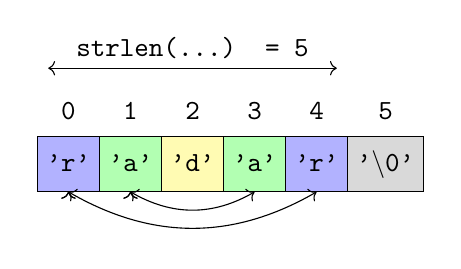
\begin{tikzpicture}[font=\ttfamily,
  array/.style={matrix of nodes,nodes={draw, minimum size=7mm},column sep=-\pgflinewidth, row sep=0.5mm, nodes in empty cells,text height=1.5ex, text depth=.25ex,
    row 1/.style={nodes={draw=none, fill=none, minimum size=5mm}},
    row 2 column 1/.style={nodes={fill=blue!30}},
    row 2 column 5/.style={nodes={fill=blue!30}},
    row 2 column 2/.style={nodes={fill=green!30}},
    row 2 column 4/.style={nodes={fill=green!30}},
    row 2 column 3/.style={nodes={fill=yellow!30}},
    row 2 column 6/.style={nodes={fill=gray!30}},
}]

\matrix[array] (array) {
 0 & 1 & 2 & 3 & 4 & 5 \\
 'r' & 'a'  &  'd'  & 'a'  & 'r' & '\textbackslash{}0' \\ };

\draw[<->]([yshift=+3mm]array-1-1.north west) -- node[above] {strlen(...) = 5} ([yshift=+3mm]array-1-5.north east);

\draw[<->] (array-2-1.south) edge [bend right] (array-2-5.south);
\draw[<->] (array-2-2.south) edge [bend right] (array-2-4.south);

\end{tikzpicture}
\end{document}
